\documentclass[11pt]{article}
\usepackage[margin=1in]{geometry}
\usepackage{amsmath,amssymb}
\usepackage{enumitem}
\usepackage{booktabs}
\usepackage{bm}
\usepackage{graphicx}
\graphicspath{{figures/}}

\newcommand{\X}{{\bm X}}

\pagestyle{plain}

\begin{document}

\begin{center}
{\Large \textbf{PS200C: Quantitative Methods}} \\[6pt]
{\large In-class Activity 10: Sensitivity --- Reading and Arguing}
\end{center}

\vspace{4pt}
\noindent\textbf{Name:} \hrulefill

\vspace{12pt}

%%% SETUP
\noindent\textbf{Setup.}  Recall the Darfur study from class: outcome \textit{PeaceIndex} (0--1); treatment \textit{DirectHarm}; adjustment for village and gender. The augmented regression table:

\medskip
\begin{center}
\begin{tabular}{lrrrrrr}
\toprule
Treatment & Est. & SE & $t$ & $R^2_{Y\sim D\mid \X}$ & RV & $\mathrm{RV}_{\alpha=0.05}$ \\
\midrule
\textit{Directly Harmed} & 0.097 & 0.023 & 4.18 & 2.2\% & 13.9\% & 7.6\% \\
\bottomrule
\end{tabular}
\end{center}
\medskip

\noindent $\mathrm{df} = 783$.  Bound from \textit{female} ($1\times$): $R^2_{Y\sim Z \mid D, \X} \leq 12\%$, $R^2_{D\sim Z \mid \X} \leq 1\%$.

\vspace{14pt}

%%% Q1 — plain English
\noindent\textbf{Question 1: Reading the table.}  Answer in one sentence each.

\medskip
\begin{enumerate}[label=(\alph*)]
\item What does $\mathrm{RV} = 13.9\%$ tell us about the Darfur result?
\vspace{3.5cm}

\item What does $\mathrm{RV}_{\alpha=0.05} = 7.6\%$ tell us, and why is it smaller than the RV?
\vspace{4cm}

\item What does $R^2_{Y\sim D \mid \X} = 2.2\%$ tell us about the role of confounding in this setting?
\vspace{2.5cm}
\end{enumerate}

\newpage

%%% Q2 — applied: reading the contour
\noindent\textbf{Question 2: Reading the contour.}  Below is the partial-$R^2$ sensitivity contour for the Darfur estimate.  Each line is the adjusted point estimate at the corresponding pair $(R^2_{D\sim Z\mid\X},\, R^2_{Y\sim Z\mid D,\X})$.  Diamond markers indicate hypothesized confounders $1\times$, $2\times$, and $3\times$ as strong as \textit{female} in their associations with both $D$ and $Y$.

\begin{center}
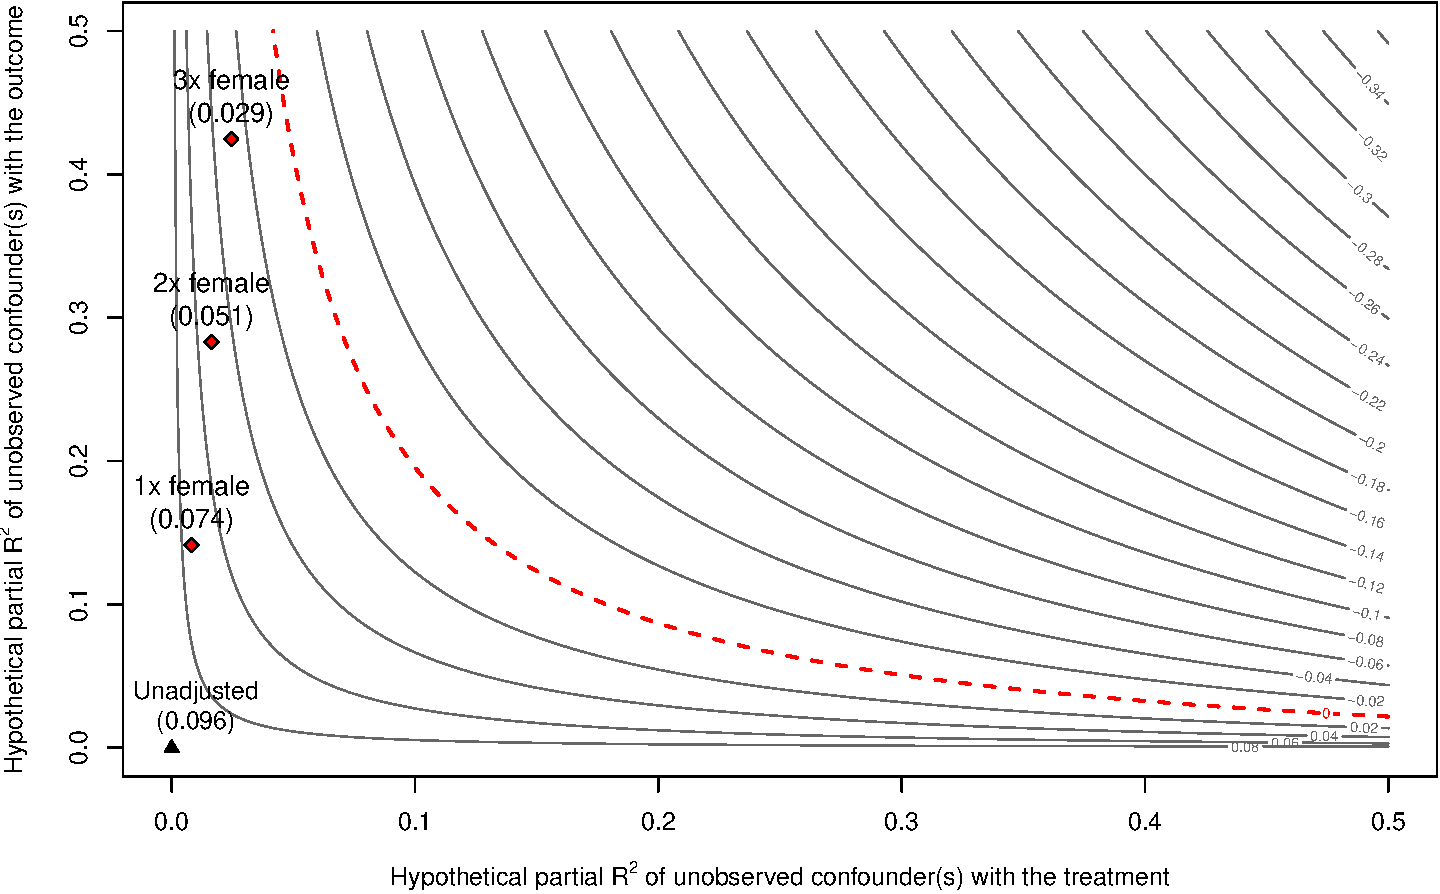
\includegraphics[width=.7\textwidth]{r2contour_female.pdf}
\end{center}

\begin{enumerate}[label=(\alph*)]
\item If unobserved confounding is twice as strongly related to the exposure (violence) and the outcome (peace index) as \textit{female} is, then how would adjusting for such unobserved confounding change the estimated effect?  Would it change your research conclusion?
\vspace{4cm}

\item This contour shows what \emph{would} happen \emph{if} confounding were $k\times$ as strong as \textit{female}.  Why is it not sufficient to just show this (or any other benchmark)? What more needs to be argued for it to be meaningful?
\vspace{2.5cm}
\end{enumerate}

%%% Q3 — spot the abuse + new scenario
% \noindent\textbf{Question 3: Spot the abuse, and what would you want?}

% \medskip
% \begin{enumerate}[label=(\alph*)]
% \item A coauthor reports: \textit{``Our RV is 12\% --- pretty high --- so we don't have to worry about unobserved confounding.''}  In one or two sentences, say what's wrong with this.
% \vspace{4cm}

% \item A new paper claims a positive effect of some treatment $D$ on outcome $Y$, adjusting for some $\X$. The published table shows $\mathrm{RV} = 4\%$, $\mathrm{RV}_{\alpha=0.05} = 2\%$, $R^2_{Y\sim D \mid \X} = 0.5\%$, and \emph{no} bounding analysis. As a reader, what would you want to see from the authors before believing the result holds?
% \vspace{6cm}
%\end{enumerate}

\end{document}
